\documentclass[floatsintext,man]{apa6}

\usepackage{amssymb,amsmath}
\usepackage{ifxetex,ifluatex}
\usepackage{fixltx2e} % provides \textsubscript
\ifnum 0\ifxetex 1\fi\ifluatex 1\fi=0 % if pdftex
  \usepackage[T1]{fontenc}
  \usepackage[utf8]{inputenc}
\else % if luatex or xelatex
  \ifxetex
    \usepackage{mathspec}
    \usepackage{xltxtra,xunicode}
  \else
    \usepackage{fontspec}
  \fi
  \defaultfontfeatures{Mapping=tex-text,Scale=MatchLowercase}
  \newcommand{\euro}{€}
\fi
% use upquote if available, for straight quotes in verbatim environments
\IfFileExists{upquote.sty}{\usepackage{upquote}}{}
% use microtype if available
\IfFileExists{microtype.sty}{\usepackage{microtype}}{}

% Table formatting
\usepackage{longtable, booktabs}
\usepackage{lscape}
% \usepackage[counterclockwise]{rotating}   % Landscape page setup for large tables
\usepackage{multirow}		% Table styling
\usepackage{tabularx}		% Control Column width
\usepackage[flushleft]{threeparttable}	% Allows for three part tables with a specified notes section
\usepackage{threeparttablex}            % Lets threeparttable work with longtable

% Create new environments so endfloat can handle them
% \newenvironment{ltable}
%   {\begin{landscape}\begin{center}\begin{threeparttable}}
%   {\end{threeparttable}\end{center}\end{landscape}}

\newenvironment{lltable}
  {\begin{landscape}\begin{center}\begin{ThreePartTable}}
  {\end{ThreePartTable}\end{center}\end{landscape}}




% The following enables adjusting longtable caption width to table width
% Solution found at http://golatex.de/longtable-mit-caption-so-breit-wie-die-tabelle-t15767.html
\makeatletter
\newcommand\LastLTentrywidth{1em}
\newlength\longtablewidth
\setlength{\longtablewidth}{1in}
\newcommand\getlongtablewidth{%
 \begingroup
  \ifcsname LT@\roman{LT@tables}\endcsname
  \global\longtablewidth=0pt
  \renewcommand\LT@entry[2]{\global\advance\longtablewidth by ##2\relax\gdef\LastLTentrywidth{##2}}%
  \@nameuse{LT@\roman{LT@tables}}%
  \fi
\endgroup}


  \usepackage{graphicx}
  \makeatletter
  \def\maxwidth{\ifdim\Gin@nat@width>\linewidth\linewidth\else\Gin@nat@width\fi}
  \def\maxheight{\ifdim\Gin@nat@height>\textheight\textheight\else\Gin@nat@height\fi}
  \makeatother
  % Scale images if necessary, so that they will not overflow the page
  % margins by default, and it is still possible to overwrite the defaults
  % using explicit options in \includegraphics[width, height, ...]{}
  \setkeys{Gin}{width=\maxwidth,height=\maxheight,keepaspectratio}
\ifxetex
  \usepackage[setpagesize=false, % page size defined by xetex
              unicode=false, % unicode breaks when used with xetex
              xetex]{hyperref}
\else
  \usepackage[unicode=true]{hyperref}
\fi
\hypersetup{breaklinks=true,
            pdfauthor={},
            pdftitle={Active transitive inference: When learner control facilitates integrative encoding},
            colorlinks=true,
            citecolor=blue,
            urlcolor=blue,
            linkcolor=black,
            pdfborder={0 0 0}}
\urlstyle{same}  % don't use monospace font for urls

\setlength{\parindent}{0pt}
%\setlength{\parskip}{0pt plus 0pt minus 0pt}

\setlength{\emergencystretch}{3em}  % prevent overfull lines


% Manuscript styling
\captionsetup{font=singlespacing,justification=justified}
\usepackage{csquotes}
\usepackage{upgreek}



\usepackage{tikz} % Variable definition to generate author note

% fix for \tightlist problem in pandoc 1.14
\providecommand{\tightlist}{%
  \setlength{\itemsep}{0pt}\setlength{\parskip}{0pt}}

% Essential manuscript parts
  \title{Active transitive inference: When learner control facilitates
integrative encoding}

  \shorttitle{Active transitive inference}


  \author{Douglas B. Markant\textsuperscript{1}}

  % \def\affdep{{""}}%
  % \def\affcity{{""}}%

  \affiliation{
    \vspace{0.5cm}
          \textsuperscript{1} Department of Psychological Science, University of North Carolina at
Charlotte  }

  \authornote{
    Douglas B. Markant, Department of Psychological Science, University of
    North Carolina at Charlotte.
    
    Correspondence concerning this article should be addressed to Douglas B.
    Markant, Department of Psychological Science, Colvard South Building,
    UNC Charlotte, 9201 University City Blvd., Charlotte, NC 28223. E-mail:
    \href{mailto:dmarkant@uncc.edu}{\nolinkurl{dmarkant@uncc.edu}}
  }


  \abstract{Research in education and psychology has shown that ``active learning''
improves learning outcomes over passive conditions. Recent work suggests
that one explanation for these findings is that learner control improves
episodic memory for study experiences. It is less clear how active
learning impacts the integration of those experiences into flexible,
generalizable knowledge. This study used a novel active transitive
inference task to investigate how people learn a relational hierarchy
through self-directed selection of premises. Active control improved
memory for studied premises as well as transitive inferences involving
items that were never experienced together. Moreover, active learners
exhibited systematic search, generating sequences of overlapping
premises that facilitate relational integration. Critically, however,
advantages from active control were not universal: Only participants
with higher working memory capacity benefited from the opportunity to
select data. These findings provide striking evidence that active
control enhances integrative encoding, but only among individuals with
sufficient cognitive resources.}
  \keywords{active learning, transitive inference, inference, memory, information
search \\

    
  }




  \usepackage{color}
  \usepackage{soul}
  \usepackage{float}
  \floatplacement{figure}{t}

\usepackage{amsthm}
\newtheorem{theorem}{Theorem}[section]
\newtheorem{lemma}{Lemma}[section]
\theoremstyle{definition}
\newtheorem{definition}{Definition}[section]
\newtheorem{corollary}{Corollary}[section]
\newtheorem{proposition}{Proposition}[section]
\theoremstyle{definition}
\newtheorem{example}{Example}[section]
\theoremstyle{definition}
\newtheorem{exercise}{Exercise}[section]
\theoremstyle{remark}
\newtheorem*{remark}{Remark}
\newtheorem*{solution}{Solution}
\begin{document}

\maketitle

\setcounter{secnumdepth}{0}



How does the opportunity to control a learning experience alter
subsequent memory of it? Recent research has shown that active control
over learning enhances episodic memory for experienced material compared
to passive observation of the same information (D. Markant, DuBrow,
Davachi, \& Gureckis, 2014; Voss, Gonsalves, Federmeier, Tranel, \&
Cohen, 2011). This enhancement can arise from a number of mechanisms,
including improved attentional coordination, metacognitive monitoring,
or changes in encoding associated with volitional control (for a review,
see D. Markant, Ruggeri, Gureckis, \& Xu, 2016).

It is less clear how active control affects the integration of studied
material into flexible, generalizable knowledge. Previous comparisons of
active and passive study have focused on memorization of independent,
unrelated items (e.g., images of objects). Other work has revealed
improved generalization from active information selection when learning
categorical rules (D. Markant \& Gureckis, 2014) or causal relationships
(Steyvers, Tenenbaum, Wagenmakers, \& Blum, 2003). However, these latter
studies cannot answer a crucial question about the cause of these
advantages: Do they reflect better memory for experienced information
itself (which then supports generalization later on) or the formation of
relational knowledge that abstracts away from that experience? Following
Zeithamova, Schlichting, and Preston (2012), these alternatives can be
mapped onto two types of memory formation: \emph{elemental encoding} of
stimuli or associations that are directly experienced, and
\emph{integrative encoding} through which disparate study episodes are
bound together into a unified representation. Existing research has
established that active control enhances elemental encoding in a variety
of contexts, but its impact on integrative encoding remains unclear.

The present study examined the effects of active control in a well-known
example of generalization from memory: transitive inference (TI). In TI
people learn about an ordered hierarchy (e.g., A \textless{} B
\textless{} C) by studing premises comprised of adjacent items (e.g., A
\textless{} B, B \textless{} C). They are then tested on their memory
for studied pairs (\emph{recall trials}; e.g., A ? B) and their ability
to infer relationships between items that were never experienced
together (\emph{inference trials}; e.g., A ? C). Transitive inference is
a fundamental building block of reasoning and has been the subject of a
wealth of past research, yet it has always been studied under passive
conditions in which control is absent. This study introduces a novel
\emph{active transitive inference} task in which participants chose
which premises to study during learning. Their goal was to learn the
\enquote{chain of command} at a set of 9-person companies, where each
premise included an employee and their direct supervisor (represented by
face images). In a passive control condition participants experienced
the same procedure but made no study decisions.

Based on prior work active selection was expected to improve recall of
studied premises relative to passive study. Active control was also
predicted to improve accuracy on inference trials, but this advantage
might arise from two distinct mechanisms. Enhanced elemental encoding of
premises should bolster retrieval during inference, allowing
participants to reason across overlapping pairs. Alternatively, active
control may enhance integrative encoding during study, aiding the
formation of a unified representation of the hierachy. Importantly,
these processes predict distinct relationships between performance and
the distance between test items (see below), making TI ideally suited to
examine how learner control changes the representation of studied
material.

\subsection{Elemental vs.~integrative encoding in transitive
inference}\label{elemental-vs.integrative-encoding-in-transitive-inference}

It has long been recognized that multiple mechanisms can support TI,
which for the present purposes can be distinguished by their dependence
on elemental or integrative encoding. Elemental encoding-based inference
occurs by reactivating studied premises and reasoning across overlapping
relations at test (D. Kumaran \& McClelland, 2012). In this case,
successful inference hinges on robust encoding of studied pairs to
ensure later retrieval. Elemental encoding-based inference implies that
greater distances between test items will lengthen response times since
more intervening pairs must be traversed, and decrease accuracy since
there are more opportunities for retrieval errors along the way.

In contrast, integrative encoding-based accounts of TI postulate the
formation of a unified representation during study (Dusek \& Eichenbaum,
1997; Hummel \& Holyoak, 2001; Shohamy \& Wagner, 2008; Zeithamova \&
Preston, 2010). By combining information from studied pairs, people
induce a spatial (De Soto, London, \& Handel, 1965; Huttenlocher, 1968)
or propositional (Hummel \& Holyoak, 2001; Trabasso, Riley, \& Wilson,
1975) representation in which items are mapped onto an integrated
ordinal dimension. Inference then simply entails comparing the positions
of any two items along that dimension. Importantly, accuracy should
\emph{increase} (and response time decrease) with inferential distance,
as items that are further apart on that latent dimension are easier to
distinguish. Such \emph{symbolic distance effects} are a hallmark of
integrative encoding (Acuna, Sanes, \& Donoghue, 2002; Moyer \&
Landauer, 1967).

Although alternative forms of associative or reinforcement learning may
also support TI (Frank, Rudy, Levy, \& O'Reilly, 2005; Von Fersen,
Wynne, Delius, \& Staddon, 1991), the construction of a propositional
representation is especially likely when participants are aware there is
an underlying hierarchy to be learned (Lazareva \& Wasserman, 2010;
Moses, Villate, \& Ryan, 2006). Accuracy is also higher among
participants who report post-task awareness of the hierarchy (Martin \&
Alsop, 2004), who are informed prior to training (Greene, Spellman,
Levy, Dusek, \& Eichenbaum, 2001; Dharshan Kumaran \& Ludwig, 2013;
Libben \& Titone, 2008; C. Smith \& Squire, 2005), or when stimuli evoke
hierarchical schemas (Dharshan Kumaran, 2013; Moses, Ostreicher, \&
Ryan, 2010). The use of propositional representations is also supported
by evidence that inference depends on working memory capacity (WMC)
(Fales et al., 2003; D. Titone, Ditman, Holzman, Eichenbaum, \& Levy,
2004), particularly when participants are aware of the hierarchy (Libben
\& Titone, 2008). In sum, integrative encoding is typically associated
with superior generalization, but also depends on explicit awareness and
incurs additional cognitive costs during study.

\subsection{Learner control and integrative
encoding}\label{learner-control-and-integrative-encoding}

Transitive inference is an ideal setting to examine whether active
control has broader benefits for memory formation beyond enriched
elemental encoding of the study experience. A principal reason to expect
enhanced integrative encoding is that people may use their current
knowledge of the hierarchy to direct their own learning. By assessing
what they already know, learners may better evaluate which option will
be informative and, in turn, more effectively allocate their study time.
At the same time, this process might involve additional demands that
depend on individual differences in working memory capacity. To evaluate
this prediction a measurement of operation span was included in addition
to the TI task.

The active TI task was also designed to explore how people decide to
select premises. Passive training often incorporates scaffolding whereby
overlapping pairs are experienced in direct succession, a procedure that
speeds learning relative to random presentation (G. S. Halford, 1984;
Waltz et al., 2004). If studying nearby premises aids relational
integration, active learners may similarly benefit from choosing such
options. Each active selection therefore involved a choice between a
\emph{near} and \emph{far} option which differed in their distance from
the pair studied on the previous trial.

\section{Experiment}\label{experiment}

The methods described below were approved by the Institutational Review
Board at UNC Charlotte (IRB \#17-0405).

\subsection{Participants}\label{participants}

\emph{N} = 100 participants (60 women; age: \emph{M} = 21.94 years,
\emph{SD} = 5.60) were recruited from the student population at UNC
Charlotte. The sample size was chosen prior to the experiment based on a
target of 25 participants for each of the four counterbalancing
conditions. Participants received either course credit or \$8 (\$4 per
session) as compensation for participating in the study. All
participants received an incentive payment based on their performance in
the first test session ranging from \$0 (\textless{} 50\% correct) to
\$5 (90--100\% correct). Payments were made in the form of Amazon gift
cards. \emph{N} = 62 participants (62\%) returned for the second
session.

\subsection{Materials}\label{materials}

Face stimuli were obtained from the 10k US Adult Faces Database
(Bainbridge, Isola, \& Oliva, 2013), a collection of images from Google
Images designed to be a representative sample of the US adult
population. The database includes subjective ratings of each face on a
number of attributes, including judgments of perceived age, emotional
affect, and memorability. For each sex, the stimulus set was filtered to
include only faces that were non-famous and which had mean ratings
within a 1-point interval centered on the midpoint of the rating scale
for perceived age, emotional affect, and memorability. Thirty-six images
(18 male, 18 female) were manually chosen from the filtered set to
ensure high image quality and the absence of other distinctive features
(e.g., jewelry, background objects). Two hierarchies were generated for
each participant by randomly sampling 18 stimuli (9 male faces, 9 female
faces).

\subsection{Procedure}\label{procedure}

There were two sessions. In the first session, participants completed
the transitive inference task followed by the operation span task. The
second session occurred 6-8 days after the first session and included
only a second run of the test phases from the transitive inference task.

\begin{figure}
\centering
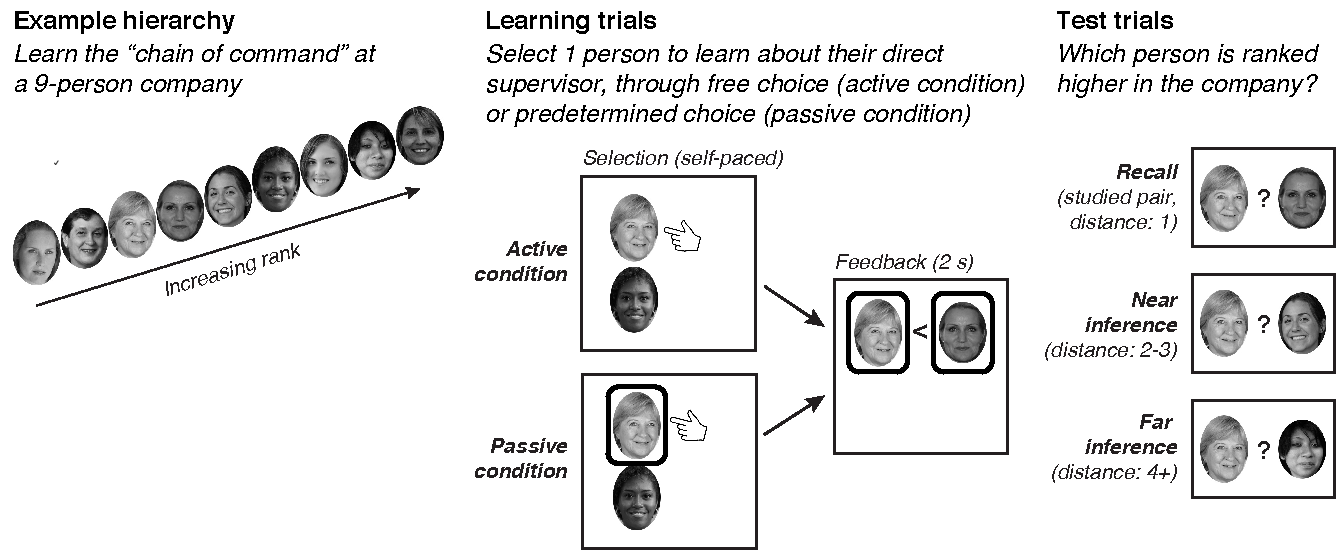
\includegraphics{figures/design.pdf}
\caption{\label{fig:unnamed-chunk-2}Transitive inference task. Participants
learned about the \enquote{chain of command} at two 9-person companies,
each made up of all men or all women (only one example shown here). In
each learning trial two individuals were presented as options. One
person was selected either through free choice (active condition) or
predetermined choice (passive condition) to receive feedback about their
direct supervisor. In each test trial participants decided which of two
individuals was ranked higher in the company, with three types of trials
depending on the distance between items in the hierarchy. \label{task}}
\end{figure}

\subsubsection{Transitive inference
task.}\label{transitive-inference-task.}

The transitive inference task (Figure \ref{task}) used a within-subjects
design with two rounds. Participants learned about one 9-item hierarchy
in the active condition and a second 9-item hierarchy in the passive
condition. Each hierarchy was composed of all female faces or all male
faces in order to reduce interference between study conditions. The
order of conditions and mapping of stimulus sex to condition were
counterbalanced across participants. Each round was comprised of a
learning phase (56 trials) followed by a test phase (72 trials).

Participants were instructed that the task involved learning about the
\enquote{chain of command} at two different companies. At the start of
each round all 9 images from the to-be-learned hierarchy were presented
in a horizontal array in random order. The instructions included an
example of a 3-item hierarchy in which participants learned about two
premise pairs (person A \textless{} person B, person B \textless{}
person C) and were asked to infer the transitive relation (person A
\textless{} person C). All participants were therefore aware of the
hierarchical nature of the stimuli and were explicitly instructed to
learn to judge the relative rank of individuals in the company.

\paragraph{Learning phase.}\label{learning-phase.}

The learning phase involved a series of choices between two options
corresponding to non-adjacent items in the present hierarchy (excluding
the highest item in the hierarchy, which had no superordinate item and
was never presented as a choice option). The options on the first
learning trial were any two non-adjacent items sampled at random. On all
subsequent trials, option sets were sampled such that the two options
differed in their distance from the option selected on the previous
trial: Each option set included a \emph{near} option that was 1--2
positions away from the option selected on the previous trial (either
above or below), and a \emph{far} option that was 3 or more positions
away from the option selected on the previous trial. This manipulation
of option distance was designed to test whether participants preferred
to select items based on their distance in the active condition. In the
passive condition selections were evenly divided between near and far
options.

\paragraph{Learning trials: Active
condition.}\label{learning-trials-active-condition.}

Each learning trial began with the presentation of the two options in a
vertical array in random order (Figure \ref{task}, middle). Participants
were instructed to select an option at their own pace in order to learn
that person's direct supervisor. Following their choice the unselected
option disappeared and the premise pair (selected item and feedback
item) was displayed for 2 s with both items highlighted by red borders.
The options then disappeared and the experiment immediately proceeded to
the next trial.

\paragraph{Learning trials: Passive
condition.}\label{learning-trials-passive-condition.}

In the passive condition participants did not decide which option to
select. As in the active condition, the trial began with the
presentation of two options, one of which was already highlighted with a
red border. Participants were instructed to select the highlighted
option at their own pace, at which point the trial proceeded in the same
manner as in the active condition.

\paragraph{Test phase: All
conditions.}\label{test-phase-all-conditions.}

In each test trial, two items were presented side-by-side and the
participant was asked to click on the item they judged to be ranked
higher in the hierarchy. Test responses were self-paced and there was no
time limit. The test phase was comprised of three types of trials:
\emph{recall} trials involving a choice between items from studied
premise pairs (e.g., A ? B), \emph{near inference} trials involving
items that were 2--3 positions apart (e.g., A ? C), and \emph{far
inference} trials involving items that were 4 or more positions apart
(e.g., A ? E). There were 3 blocks of 24 trials, with each block made up
of an equal number of recall, near inference, and far inference trials
presented in random order. In the second session, participants completed
a second run of the same test phase experienced during the first
session, with test pairs presented in a new random order.

\subsubsection{Operation span.}\label{operation-span.}

The operation span is a well-established measure of working memory
capacity in which participants attempt to hold a sequence of items in
memory while evaluating a set of interleaved math operations (Turner \&
Engle, 1989; Unsworth, Heitz, Schrock, \& Engle, 2005). In the version
used for this study (obtained from
\url{http://www.cognitivetools.uk/cognition/tasks/Verbal-WM/operationSpan/})
participants attempted to remember sets of digits while judging the
validity of arithmetic problems. For each math operation they first
evaluated whether an equation was correct (e.g., \emph{2 - 4 = -2}) or
incorrect (e.g., \emph{2 - 4 = 6}). This judgment was followed by the
presentation of a digit to be maintained in memory. At the end of a
trial involving multiple such steps, they then attempted to recall the
sequence of digits in the order in which they had appeared. The set size
(number of operations/digits) ranged from 2--7, presented in increasing
order. There were three trials of each set size for a total of 18
trials.

\section{Results}\label{results}

The results described below are based on data from all participants,
including those who did not return for the second session. Returning and
non-returning participants did not differ in terms of overall accuracy
on the first test, \(\Delta M = 0.04\), 95\% CI \([-0.10\), \(0.02]\),
\(t(64.03) = -1.35\), \(p = .182\), gender distribution,
\(\chi^2(1, n = 100) = 0.00\), \(p > .999\), or operation span,
\(\Delta M = 0.54\), 95\% CI \([-5.14\), \(4.06]\),
\(t(81.28) = -0.23\), \(p = .816\). Separate analyses restricted to data
from returning participants did not produce qualitatively different
results. All error bars in figures represent 95\% confidence intervals
calculated using the Cousineau-Morey method (Morey, 2008).

\subsection{Operation span}\label{operation-span}

Participants were highly accurate at evaluating the validity of the math
operations (judgment accuracy \emph{M} = 0.92, \emph{SD} = 0.06). The
operation span was scored according to the summed number of digits
recalled in the correct order, for those trials in which no errors were
made (\emph{M} = 14.86, \emph{SD} = 11.29, median = 12.50). Operation
span scores were square root transformed to correct for positive skew
and standardized prior to inclusion in the regression models described
below.

\subsection{Test performance}\label{test-performance}

\subsubsection{Accuracy}\label{accuracy}

Test responses were scored according to whether participants correctly
identified the superordinate item in each test pair (0 = incorrect, 1 =
correct). Test trials involving either endpoint of the hierarchy were
excluded since participants could rely on non-transitive strategies to
respond (e.g., the highest-ranked item was never presented as an option
on the left side of the screen). A separate analysis of test accuracy
for trials involving endpoint items is presented in the supplementary
material.

\begin{table}[tbp]
\begin{center}
\begin{threeparttable}
\caption{\label{tab:accuracy}Estimated fixed effects (relative odds ratios) from logistic regression model of test accuracy.}
\small{
\begin{tabular}{lrrr}
\toprule
Predictor & \multicolumn{1}{c}{OR} & \multicolumn{1}{c}{95\% CI-lower} & \multicolumn{1}{c}{95\% CI-upper}\\
\midrule
(Intercept) & 4.12 & 3.32 & 5.24\\
Condition [passive] & 0.76 & 0.68 & 0.84\\
Session [retest] & 0.84 & 0.74 & 0.95\\
Distance & 1.08 & 1.02 & 1.15\\
Operation span & 1.97 & 1.67 & 2.62\\
Condition [passive] x Session [retest] & 0.81 & 0.69 & 0.95\\
Condition [passive] x Distance & 0.96 & 0.88 & 1.05\\
Condition [passive] x Operation span & 0.55 & 0.49 & 0.59\\
\bottomrule
\end{tabular}
}
\end{threeparttable}
\end{center}
\end{table}

Accuracy was modeled using mixed effects logistic regression. The model
included fixed effects for condition (active/passive), session
(test/retest), distance (recall/near inference/far inference), and
operation span score (continuous), as well as pairwise interactions
between condition and session, operation span, and distance. Random
intercepts were included for participants as well as stimulus test pairs
(in order to account for any item-specific effects on memorability).
Table \ref{tab:accuracy} presents parameter estimates and confidence
intervals for fixed effects in terms of relative odds ratios
(\emph{OR}), which indicate the multiplicative change in the odds of
responding correctly given a unit change in the predictor.

Active performance was higher than passive performance in both the
immediate test (active: \emph{M} = 0.74, \emph{SD} = 0.21; passive:
\emph{M} = 0.71, \emph{SD} = 0.21; \emph{OR} = 1.31, \emph{CI} =
{[}1.13, 1.53{]}, \emph{z} = 5.01, \emph{p} \textless{} .001) and in the
retest (active: \emph{M} = 0.73, \emph{SD} = 0.21; passive: \emph{M} =
0.65, \emph{SD} = 0.21; \emph{OR} = 1.62, \emph{CI} = {[}1.34, 1.94{]},
\emph{z} = 7.26, \emph{p} \textless{} .001). Accuracy declined from the
first test to the second test in both the active condition (\emph{OR} =
0.84, \emph{CI} = {[}0.70, 1.00{]}, \emph{z} = -2.86, \emph{p} = 0.004)
and the passive condition (\emph{OR} = 0.68, \emph{CI} = {[}0.57,
0.80{]}, \emph{z} = -6.44, \emph{p} \textless{} .001). There was a
significant symbolic distance effect, such that accuracy increased with
inferential distance, in the active condition (\emph{OR} = 1.08,
\emph{CI} = {[}0.99, 1.19{]}, \emph{z} = 2.51, \emph{p} = 0.01) but not
the passive condition (\emph{OR} = 1.04, \emph{CI} = {[}0.95, 1.13{]},
\emph{z} = 1.25, \emph{p} = 0.21).

\begin{figure}
\centering
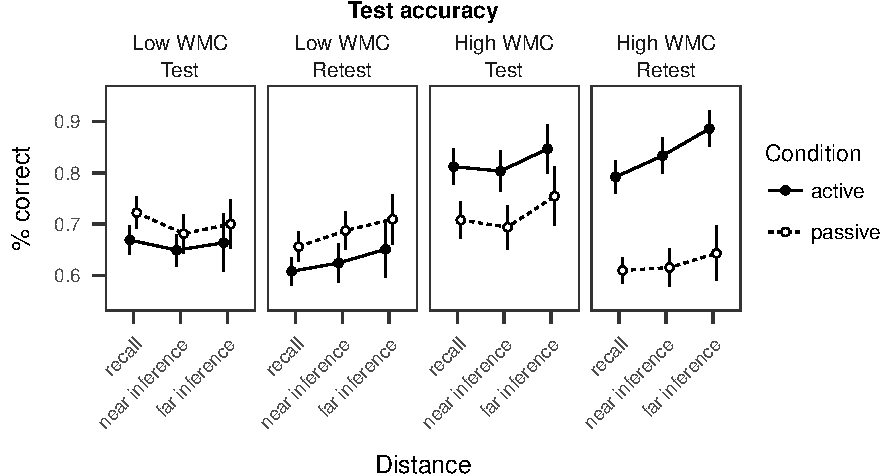
\includegraphics{active_transitive_inference_files/figure-latex/unnamed-chunk-3-1.pdf}
\caption{\label{fig:unnamed-chunk-3}Test accuracy as a function of
inferential distance and test session, following a median split on
working memory capacity (operation span scores). \label{fig_acc}}
\end{figure}

Operation span was positively related to performance in the active
condition (\emph{OR} = 1.97, \emph{CI} = {[}1.44, 2.68{]}, \emph{z} =
6.05, \emph{p} \textless{} .001) but not the passive condition
(\emph{OR} = 1.08, \emph{CI} = {[}0.79, 1.47{]}, \emph{z} = 0.68,
\emph{p} = 0.50). A median split on operation span was used to divide
participants into a low working memory group (\emph{N} = 50) and high
working memory group (\emph{N} = 50). Figure \ref{fig_acc} shows the
test performance for each group as a function of inferential distance. A
followup analysis was performed to examine differences in overall
accuracy based on this grouping (aggregating over distance levels).
Active performance exceeded passive performance in the high WMC group
(test: \emph{OR} = 1.97, \emph{CI} = {[}1.58, 2.44{]}, \emph{z} = 8.50,
\emph{p} \textless{} .001; retest: \emph{OR} = 3.48, \emph{CI} =
{[}2.65, 4.56{]}, \emph{z} = 12.57, \emph{p} \textless{} .001), but was
lower than passive performance in the low WMC group (test: \emph{OR} =
0.80, \emph{CI} = {[}0.66, 0.97{]}, \emph{z} = -3.11, \emph{p} = 0.002;
retest: \emph{OR} = 0.76, \emph{CI} = {[}0.60, 0.96{]}, \emph{z} =
-3.15, \emph{p} = 0.002). In the high WMC group there was no decline in
performance from the test to the retest in the active condition
(\emph{OR} = 0.99, \emph{CI} = {[}0.76, 1.31{]}, \emph{z} = -0.06,
\emph{p} = 0.96), but a large decrease in the passive condition
(\emph{OR} = 0.56, \emph{CI} = {[}0.45, 0.71{]}, \emph{z} = -6.71,
\emph{p} \textless{} .001). In the low WMC group performance declined
from the test to the retest in both conditions (active: \emph{OR} =
0.76, \emph{CI} = {[}0.61, 0.95{]}, \emph{z} = -3.39, \emph{p}
\textless{} .001; passive: \emph{OR} = 0.80, \emph{CI} = {[}0.64,
1.01{]}, \emph{z} = -2.59, \emph{p} = 0.010). Thus, active and passive
study had markedly different consequences depending on participants'
operation span, with active control leading to a large, sustained
advantage only among higher working memory participants.

\subsubsection{Response time}\label{response-time}

\begin{figure}
\centering
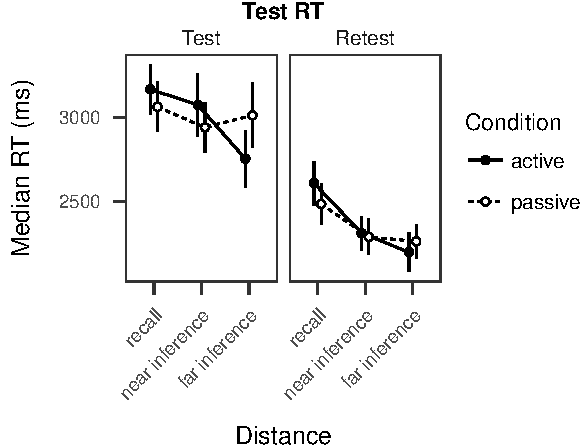
\includegraphics{active_transitive_inference_files/figure-latex/unnamed-chunk-4-1.pdf}
\caption{\label{fig:unnamed-chunk-4}Response time as a function of
inferential distance and test session). \label{fig_rt}}
\end{figure}

Median response time (RT) on test trials was modeled using mixed effects
linear regression. Figure \ref{fig_rt} shows RT as a function of
inferential distance and condition. RT decreased from the test to the
retest in both the active (test: \emph{M} = 2998, \emph{SD} = 1121;
retest: \emph{M} = 2374, \emph{SD} = 617; \(\beta\) = -695.50, \emph{CI}
= {[}-889.21, -501.79{]}, \emph{z} = -9.95, \emph{p} \textless{} .001),
and the passive condition (test: \emph{M} = 3005, \emph{SD} = 1120;
retest: \emph{M} = 2347, \emph{SD} = 722; \(\beta\) = -730.06, \emph{CI}
= {[}-923.78, -536.35{]}, \emph{z} = -10.45, \emph{p} \textless{} .001).
However, there were no differences in RT between active and passive
conditions for either the test (\(\beta\) = -7.32, \emph{CI} =
{[}-168.99, 154.34{]}, \emph{z} = -0.13, \emph{p} = 0.90) or the retest
(\(\beta\) = 27.24, \emph{CI} = {[}-178.07, 232.56{]}, \emph{z} = 0.37,
\emph{p} = 0.71), nor were there significant relationships between
operation span scores and RTs in either the active (\(\beta\) = 81.03,
\emph{CI} = {[}-128.38, 290.44{]}, \emph{z} = 1.07, \emph{p} = 0.28) or
passive condition (\(\beta\) = 127.82, \emph{CI} = {[}-81.59, 337.23{]},
\emph{z} = 1.69, \emph{p} = 0.09).

Although the two conditions did not differ in overall test RT, they
showed different relationships with inferential distance between test
items. Response times decreased with distance in the active condition in
both the test (\(\beta\) = -168.20, \emph{CI} = {[}-282.50, -53.90{]},
\emph{z} = -4.08, \emph{p} \textless{} .001) and the retest (\(\beta\) =
-167.15, \emph{CI} = {[}-312.32, -21.99{]}, \emph{z} = -3.19, \emph{p} =
0.001), whereas distance had no effect on RT in the passive condition in
either the test (\(\beta\) = -20.41, \emph{CI} = {[}-134.71, 93.89{]},
\emph{z} = -0.49, \emph{p} = 0.62) or the retest (\(\beta\) = -91.98,
\emph{CI} = {[}-326.95, 142.99{]}, \emph{z} = -1.09, \emph{p} = 0.28).
As was seen in the accuracy results above, a symbolic distance effect
was therefore apparent from RTs in the active condition only, with an
advantage for more distant inferences as compared to near inferences and
direct recall of studied premise pairs.

\subsection{Selections during
learning}\label{selections-during-learning}

The next analysis focused on participants' selections in the learning
phase and the extent to which they can account for differences in test
performance described above. Notably, study condition was not related to
selection frequency (multinomial logistic regression, likelihood ratio
test: \(\chi_{(1,7)}^2\) = 7.20, \emph{p} = 0.41), indicating that the
overall distribution of experienced premise pairs was matched across
active and passive study. Although individuals may have exhibited
idiosyncratic selection behavior in the active condition, at the
aggregate level there were no apparent differences in study frequency
from the passive condition.

Each selection trial involved a choice between a near option (1--2
positions away from the option selected on the previous trial) and a far
option (3 or more positions away). By design, the proportion of near
selections in the passive condition was approximately 50\% (\emph{M} =
0.50, \emph{SD} = 0.01). In the active condition participants had a
small but robust preference for selecting the near option (\emph{M} =
0.56, \emph{SD} = 0.07; \emph{OR} = 1.30, \emph{CI} = {[}1.21, 1.40{]},
\emph{z} = 6.86, \emph{p} \textless{} .001). As a result, the average
distance between successive selections was lower in the active condition
(\emph{M} = 2.63, \emph{SD} = 0.13) than the passive condition (\emph{M}
= 2.83, \emph{SD} = 0.13; \(M_d = -0.21\), 95\% CI \([-0.26\),
\(-0.15]\), \(t(99) = -7.53\), \(p < .001\)).

Near selections may be especially useful if they cause overlapping
premise pairs to be experienced in successive trials, which might
facilitate integrative encoding when representations of overlapping
premises are simultaneously active. I next examined whether the
preference to select near items in the active condition depended on the
distance between the near option and the item selected on the previous
trial (\(dist_{\text{near}} \in \{-2, -1, +1, +2\}\)). When
\(dist_{\text{near}}=+1\), the near option was immediately superordinate
to the previously selected item; that is, the near option had appeared
as the feedback in the previous trial.

\begin{figure}
\centering
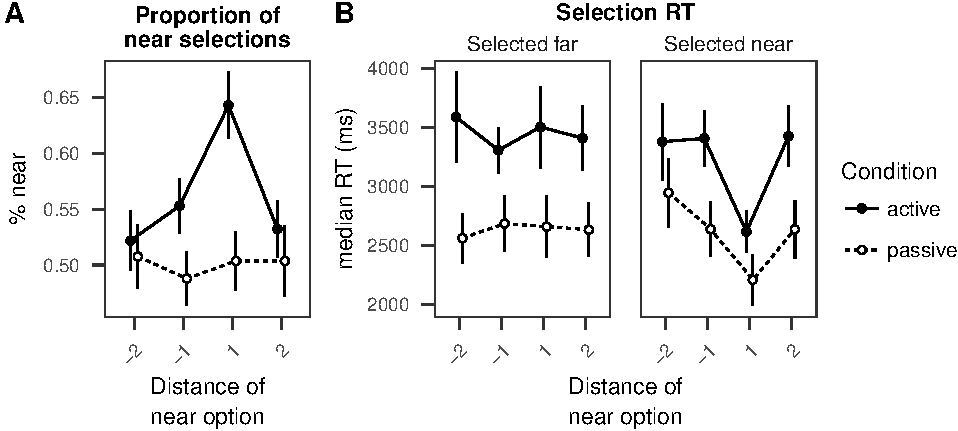
\includegraphics{active_transitive_inference_files/figure-latex/unnamed-chunk-5-1.pdf}
\caption{\label{fig:unnamed-chunk-5}A: Proportion of near selections during
learning phase. B: Median response time of selections as a function of
trial type. \label{fig_prop_near}}
\end{figure}

Figure \ref{fig_prop_near}A shows the proportion of near selections as a
function of their distance from the previous selection. In the passive
condition, by design there was an equal likelihood of selecting the near
item regardless of its distance (\(dist_{\text{near}}=-2\): \emph{M} =
0.51, \emph{SD} = 0.13; \(dist_{\text{near}}=-1\): \emph{M} = 0.49,
\emph{SD} = 0.11; \(dist_{\text{near}}=+1\): \emph{M} = 0.50, \emph{SD}
= 0.12; \(dist_{\text{near}}=+2\): \emph{M} = 0.50, \emph{SD} = 0.14.)
In the active condition, the proportion of near selections did not
differ from the passive condition when \(dist_{\text{near}}=-2\)
(\emph{M} = 0.52, \emph{SD} = 0.14; \emph{OR} = 1.05, \emph{CI} =
{[}0.86, 1.29{]}, \emph{z} = 0.63, \emph{p} = 0.53) or
\(dist_{\text{near}}=+2\) (\emph{M} = 0.53, \emph{SD} = 0.13; \emph{OR}
= 1.15, \emph{CI} = {[}0.94, 1.41{]}, \emph{z} = 1.73, \emph{p} = 0.08).
However, there was a higher proportion of near selections when
\(dist_{\text{near}}=-1\) (\emph{M} = 0.55, \emph{SD} = 0.13; \emph{OR}
= 1.29, \emph{CI} = {[}1.07, 1.56{]}, \emph{z} = 3.48, \emph{p}
\textless{} .001) or \(dist_{\text{near}}=+1\) (\emph{M} = 0.64,
\emph{SD} = 0.15; \emph{OR} = 1.75, \emph{CI} = {[}1.45, 2.11{]},
\emph{z} = 7.52, \emph{p} \textless{} .001). Within the active
condition, the proportion of near selections was markedly higher for
\(dist_{\text{near}}=+1\) than \(dist_{\text{near}}=-1\) options
(\emph{OR} = 1.45, \emph{CI} = {[}1.20, 1.75{]}, \emph{z} = 4.95,
\emph{p} \textless{} .001). Thus, participants preferred to select the
near option when it was adjacent to the option selected on the previous
trial, and this preference was strongest when the option had apppeared
as feedback in that trial. Whereas items were selected with similar
frequencies across study conditions, this result shows that participants
generated study sequences during active study in which overlapping
premises were more likely to be experienced in successive trials.

Can this tendency to select overlapping premises account for the
performance benefit in the active condition? A new model of test
accuracy was fit for the active condition which included predictors for
the proportion of near selections at each level of
\(dist_{\text{near}}\). There was no relationship between accuracy and
proportion of near selections when distance was
\(dist_{\text{near}}=-2\) (\emph{OR} = 1.02, \emph{CI} = {[}0.70,
1.48{]}, \emph{z} = 0.10, \emph{p} = 0.92), \(dist_{\text{near}}=-1\)
(\emph{OR} = 1.28, \emph{CI} = {[}0.88, 1.84{]}, \emph{z} = 1.65,
\emph{p} = 0.10), \(dist_{\text{near}}=+1\) (\emph{OR} = 0.95, \emph{CI}
= {[}0.65, 1.38{]}, \emph{z} = -0.37, \emph{p} = 0.71), or
\(dist_{\text{near}}=+2\) (\emph{OR} = 1.28, \emph{CI} = {[}0.86,
1.90{]}, \emph{z} = 1.57, \emph{p} = 0.12). The proportion of near
selections at any distance was also unrelated to operation span
(\(dist_{\text{near}}=-2\): \emph{OR} = 0.93, \emph{CI} = {[}0.80,
1.07{]}, \emph{z} = -1.34, \emph{p} = 0.18; \(dist_{\text{near}}=-1\):
\emph{OR} = 0.98, \emph{CI} = {[}0.85, 1.12{]}, \emph{z} = -0.38,
\emph{p} = 0.70; \(dist_{\text{near}}=+1\): \emph{OR} = 1.07, \emph{CI}
= {[}0.93, 1.22{]}, \emph{z} = 1.19, \emph{p} = 0.23;
\(dist_{\text{near}}=+2\): \emph{OR} = 0.98, \emph{CI} = {[}0.85,
1.14{]}, \emph{z} = -0.30, \emph{p} = 0.77). Therefore, the preference
to select overlapping options was a general one and could not on its own
account for the divergence between active and passive conditions.

\subsubsection{Response time}\label{response-time-1}

Median response times during selection were higher in the active
condition (\emph{M} = 3149, \emph{SD} = 1536) than the passive condition
(\emph{M} = 2494, \emph{SD} = 1258; \(\beta\) = 656.66, \emph{CI} =
{[}378.00, 935.32{]}, \emph{z} = 5.57, \emph{p} \textless{} .001),
confirming that the need to make a selection decision was associated
with an additional processing load. In addition, selection RT in the
active condition was positively related to operation span (\(\beta\) =
511.42, \emph{CI} = {[}190.74, 832.10{]}, \emph{z} = 3.77, \emph{p}
\textless{} .001), whereas there was no relationship between operation
span and selection RT in the passive condition (\(\beta\) = 205.03,
\emph{CI} = {[}-115.65, 525.71{]}, \emph{z} = 1.51, \emph{p} = 0.13).
Thus, high WMC participants who tended to have high accuracy in the
active condition also tended to take longer when making selection
decisions.

Lastly, I examined how selection RT depended on the distance of the near
option, which was shown in the previous section to be strongly preferred
when it was immediately superordinate to the option selected in the last
trial (\(dist_{\text{near}}=+1\)). Figure \ref{fig_prop_near}B shows
median RT on trials in which the far option was selected (left) and
trials in which the near option was selected (right). A three-way
repeated measures ANOVA was performed with condition (active/passive),
near option distance (\(-2/-1/+1/+2\)), and selection (near/far) as
within-subjects factors. In addition to the main effect of condition
noted above (\(F(1, 1483) = 121.71\), \(\mathit{MSE} = 1,648,172.16\),
\(p < .001\), \(\hat{\eta}^2_G = .076\)), there was a main effect of
selection (\(F(1, 1483) = 4.46\), \(\mathit{MSE} = 1,648,172.16\),
\(p = .035\), \(\hat{\eta}^2_G = .003\)) with RT lower when the near
option was selected. There was also a main effect of near option
distance (\(F(3, 1483) = 6.22\), \(\mathit{MSE} = 1,648,172.16\),
\(p < .001\), \(\hat{\eta}^2_G = .012\)) and an interaction between
selection and near distance (\(F(3, 1483) = 7.79\),
\(\mathit{MSE} = 1,648,172.16\), \(p < .001\),
\(\hat{\eta}^2_G = .016\)). Post-hoc comparisons indicated that when the
far was option was selected (Figure \ref{fig_prop_near}B, left), there
were no differences in RT as a function of distance in either condition
(Tukey HSD, all \emph{p} \textgreater{} .4). When the near option was
selected in the active condition (Figure \ref{fig_prop_near}B, right),
\(dist_{\text{near}}=+1\) options were selected faster than all other
types (all \emph{p} \textless{} .001) but there were no other
differences between option distances. In the passive condition,
\(dist_{\text{near}}=+1\) options were selected faster than
\(dist_{\text{near}}=-2\) options (\emph{p} \textless{} .001) but there
were no other differences between near option distances. In sum, the
preference to select the near option when it had appeared as feedback on
the previous trial was also evident in faster selection decisions. The
primacy of \(dist_{\text{near}}=+1\) options was even apparent in the
passive condition in which there was no selection decision to be made.

\section{Discussion}\label{discussion}

This study used a novel TI task to examine whether active control aids
the integration of relational knowledge during study. Control over the
selection of premise pairs improved performance relative to passive
study in both an immediate test and a retest one week later. Symbolic
distance effects observed in the active condition strongly imply that
this benefit resulted from enhanced integrative encoding, such that
active learners relied on an integrated representation of the hierarchy
rather than sequential reactivation of premise pairs at test (Acuna et
al., 2002; Zeithamova et al., 2012). The absence of such effects
following passive study suggests that integrative encoding was less
prevalent when the same participants lacked the opportunity to select
data.

Active control did not benefit all learners, however, as working memory
capacity strongly predicted accuracy in the active condition. Among
higher WMC participants, active control produced a \textasciitilde{}10\%
initial advantage over passive study (increasing past 20\% in the
retest) and sustained performance across sessions. WMC was unrelated to
accuracy in the passive condition, a finding that conflicts with reports
that WMC moderates TI under experimenter-controlled conditions (e.g.,
Libben \& Titone, 2008). This discrepancy may be due to the relative
difficulty of passive study in the present task. Previous studies have
typically involved smaller hierarchies (ranging from 3--6 items) and
scaffolded training sequences. For instance, Libben and Titone (2008)
used clustered sequences in which participants were likely to experience
overlapping pairs. With larger hierarchies and sequences with relatively
high distances between successive premises, the passive condition used
here may have been comparatively difficult even for participants with
higher WMC.

This study provides the first evidence of systematic search in TI:
Participants strongly preferred to select options that appeared as
feedback on the previous trial (\(dist_{\text{near}}=+1\)). Participants
thereby naturally generated \enquote{chained} sequences of overlapping
pairs which tend to improve performance in passive conditions relative
to random presentation (Andrews, 2010; G. S. Halford, 1984; Waltz et
al., 2004). This preference was widespread: 82 of 100 participants chose
the \(dist_{\text{near}}=+1\) option in more than half of trials in
which one appeared, and the proportion of near selections was unrelated
to WMC. Participants were also faster to select
\(dist_{\text{near}}=+1\) options in both study conditions. At present
it is unclear what drives this selection preference. People may ascribe
higher value to chained sequences if they have metacognitive awareness
of how to sequence study when learning about related materials
(Wahlheim, Dunlosky, \& Jacoby, 2011). However, preferring items from
the previous trial might also be explained by simpler forms of priming
(Chun \& Nakayama, 2000) or attention to recurring visual features
(Zhao, Al-Aidroos, \& Turk-Browne, 2013).

Selection of overlapping premises should promote integrative encoding,
yet not everyone benefited from it, suggesting that differences in study
sequences alone cannot account for active performance. One possibility
is that only high WMC individuals capitalize on chained sequences
because they maintain representations of premises from trial to trial.
Alternatively, high WMC individuals may construct a representation of
the hierarchy to decide which option will be useful (e.g., choosing to
learn about the option whose rank is more uncertain). This
interpretation is consistent with the finding that overall selection RT
was positively related to WMC, reflecting additional time before it was
possible to encode feedback information (Maybery, Bain, \& Halford,
1986). Further work is necessary to determine whether this goal-directed
evaluation of options' usefulness during selection contributes to the
active advantage among high WMC individuals.

These findings offer a new perspective on TI research, which heretofore
has focused on experimenter-designed (and somewhat artisanal) training
sequences. This ignores people's ability to gather information during
knowledge formation and, as demonstrated here, can underestimate the
efficiency of learning when control is possible (Gureckis \& Markant,
2012). Morever, the present findings have implications for the value of
active control in relational learning more generally. The opportunity to
select data may not enhance integrative encoding if a person is unable
to bring to mind related experiences. For those individuals, active
learning may be most effective in concert with memory aids that support
comparison and integration (Son, Smith, \& Goldstone, 2011).

Finally, it is important to note that participants were aware that there
was an underlying hierarchy to be learned. Awareness influences strategy
use in TI (C. Smith \& Squire, 2005) and it is unknown how active
control might affect performance in its absence. It is likely that
active study enhances elemental encoding in such conditions, perhaps due
to the mere opportunity for volitional control (Murty, DuBrow, \&
Davachi, 2015) or additional metacognitive processing (e.g., retrieval
practice, Kornell, Klein, \& Rawson, 2015). An intriguing further
possibility is that active control increases the likelihood of becoming
aware of the hierarchy by directing attention to abstract relationships
across study episodes (Henriksson \& Enkvist, 2016). This would lend
support to the broader notion that active learning not only enriches
memory for experienced materials, but also fosters self-directed
discovery of abstract knowledge.

\section{Acknowledgements}\label{acknowledgements}

The author thanks Meagan Padro, Michele Xiong, Delanie Postma, Arielle
Little, and Sunidhi Gupta for assistance with data collection and
literature review.

\newpage

\section{References}\label{references}

\begingroup
\setlength{\parindent}{-0.5in} \setlength{\leftskip}{0.5in}

\hypertarget{refs}{}
\hypertarget{ref-acuna2002cognitive}{}
Acuna, B. D., Sanes, J. N., \& Donoghue, J. P. (2002). Cognitive
mechanisms of transitive inference. \emph{Experimental Brain Research},
\emph{146}(1), 1--10.

\hypertarget{ref-andrews2010belief}{}
Andrews, G. (2010). Belief-based and analytic processing in transitive
inference depends on premise integration difficulty. \emph{Memory \&
Cognition}, \emph{38}(7), 928--940.

\hypertarget{ref-bainbridge2013intrinsic}{}
Bainbridge, W. A., Isola, P., \& Oliva, A. (2013). The intrinsic
memorability of face photographs. \emph{Journal of Experimental
Psychology: General}, \emph{142}(4), 1323.

\hypertarget{ref-chun2000functional}{}
Chun, M. M., \& Nakayama, K. (2000). On the functional role of implicit
visual memory for the adaptive deployment of attention across scenes.
\emph{Visual Cognition}, \emph{7}(1-3), 65--81.

\hypertarget{ref-de1965social}{}
De Soto, C. B., London, M., \& Handel, S. (1965). Social reasoning and
spatial paralogic. \emph{Journal of Personality and Social Psychology},
\emph{2}(4), 513.

\hypertarget{ref-dusek1997hippocampus}{}
Dusek, J. A., \& Eichenbaum, H. (1997). The hippocampus and memory for
orderly stimulus relations. \emph{Proceedings of the National Academy of
Sciences}, \emph{94}(13), 7109--7114.

\hypertarget{ref-fales2003working}{}
Fales, C. L., Knowlton, B. J., Holyoak, K. J., Geschwind, D. H.,
Swerdloff, R. S., \& Gonzalo, I. G. (2003). Working memory and
relational reasoning in Klinefelter syndrome. \emph{Journal of the
International Neuropsychological Society}, \emph{9}(6), 839--846.

\hypertarget{ref-frank2005logic}{}
Frank, M. J., Rudy, J. W., Levy, W. B., \& O'Reilly, R. C. (2005). When
logic fails: Implicit transitive inference in humans. \emph{Memory \&
Cognition}, \emph{33}(4), 742--750.

\hypertarget{ref-greene2001relational}{}
Greene, A. J., Spellman, B. A., Levy, W. B., Dusek, J. A., \&
Eichenbaum, H. B. (2001). Relational learning with and without
awareness: Transitive inference using nonverbal stimuli in humans.
\emph{Memory \& Cognition}, \emph{29}(6), 893--902.

\hypertarget{ref-Gureckis-2012-PPS}{}
Gureckis, T. M., \& Markant, D. B. (2012). Self-directed learning: A
cognitive and computational perspective. \emph{Perspectives on
Psychological Science}, \emph{7}(5), 464--481.

\hypertarget{ref-halford1984can}{}
Halford, G. S. (1984). Can young children integrate premises in
transitivity and serial order tasks? \emph{Cognitive Psychology},
\emph{16}(1), 65--93.

\hypertarget{ref-henriksson2016learning}{}
Henriksson, M. P., \& Enkvist, T. (2016). Learning from observation,
feedback, and intervention in linear and nonlinear task environments.
\emph{The Quarterly Journal of Experimental Psychology}, 1--57.

\hypertarget{ref-hummel2001process}{}
Hummel, J. E., \& Holyoak, K. J. (2001). A process model of human
transitive inference. In \emph{Spatial schemas in abstract thought} (pp.
279--305).

\hypertarget{ref-huttenlocher1968constructing}{}
Huttenlocher, J. (1968). Constructing spatial images: A strategy in
reasoning. \emph{Psychological Review}, \emph{75}(6), 550.

\hypertarget{ref-kornell2015retrieval}{}
Kornell, N., Klein, P. J., \& Rawson, K. A. (2015). Retrieval attempts
enhance learning, but retrieval success (versus failure) does not
matter. \emph{Journal of Experimental Psychology: Learning, Memory, and
Cognition}, \emph{41}(1), 283.

\hypertarget{ref-kumaran2013schema}{}
Kumaran, D. (2013). Schema-driven facilitation of new hierarchy learning
in the transitive inference paradigm. \emph{Learning \& Memory},
\emph{20}(7), 388--394.

\hypertarget{ref-kumaran2013transitivity}{}
Kumaran, D., \& Ludwig, H. (2013). Transitivity performance, relational
hierarchy knowledge and awareness: Results of an instructional framing
manipulation. \emph{Hippocampus}, \emph{23}(12), 1259--1268.

\hypertarget{ref-kumaran2012generalization}{}
Kumaran, D., \& McClelland, J. (2012). Generalization through the
recurrent interaction of episodic memories: A model of the hippocampal
system. \emph{Psychological Review}, \emph{119}(3), 573.

\hypertarget{ref-lazareva2010nonverbal}{}
Lazareva, O. F., \& Wasserman, E. A. (2010). Nonverbal transitive
inference: Effects of task and awareness on human performance.
\emph{Behavioural Processes}, \emph{83}(1), 99--112.

\hypertarget{ref-libben2008role}{}
Libben, M., \& Titone, D. (2008). The role of awareness and working
memory in human transitive inference. \emph{Behavioural Processes},
\emph{77}(1), 43--54.

\hypertarget{ref-markant2014select}{}
Markant, D., \& Gureckis, T. M. (2014). Is it better to select or to
receive? Learning via active and passive hypothesis testing.
\emph{Journal of Experimental Psychology: General}, \emph{143}(1),
94--122.

\hypertarget{ref-markant2014deconstructing}{}
Markant, D., DuBrow, S., Davachi, L., \& Gureckis, T. M. (2014).
Deconstructing the effect of self-directed study on episodic memory.
\emph{Memory \& Cognition}, \emph{42}(8), 1211--1224.

\hypertarget{ref-markant2016enhanced}{}
Markant, D., Ruggeri, A., Gureckis, T. M., \& Xu, F. (2016). Enhanced
memory as a common effect of active learning. \emph{Mind, Brain, and
Education}, \emph{10}(3), 142--152.

\hypertarget{ref-martin2004transitive}{}
Martin, N., \& Alsop, B. (2004). Transitive inference and awareness in
humans. \emph{Behavioural Processes}, \emph{67}(2), 157--165.

\hypertarget{ref-maybery1986information}{}
Maybery, M. T., Bain, J. D., \& Halford, G. S. (1986).
Information-processing demands of transitive inference. \emph{Journal of
Experimental Psychology: Learning, Memory, and Cognition}, \emph{12}(4),
600--613.

\hypertarget{ref-morey2008confidence}{}
Morey, R. D. (2008). Confidence intervals from normalized data: A
correction to Cousineau (2005). \emph{Reason}, \emph{4}(2), 61--64.

\hypertarget{ref-moses2010relational}{}
Moses, S. N., Ostreicher, M. L., \& Ryan, J. D. (2010). Relational
framework improves transitive inference across age groups.
\emph{Psychological Research PRPF}, \emph{74}(2), 207--218.

\hypertarget{ref-moses2006investigation}{}
Moses, S. N., Villate, C., \& Ryan, J. D. (2006). An investigation of
learning strategy supporting transitive inference performance in humans
compared to other species. \emph{Neuropsychologia}, \emph{44}(8),
1370--1387.

\hypertarget{ref-moyer1967time}{}
Moyer, R. S., \& Landauer, T. K. (1967). Time required for judgements of
numerical inequality. \emph{Nature}, \emph{215}, 1519--1520.

\hypertarget{ref-murty2015simple}{}
Murty, V. P., DuBrow, S., \& Davachi, L. (2015). The simple act of
choosing influences declarative memory. \emph{The Journal of
Neuroscience}, \emph{35}(16), 6255--6264.

\hypertarget{ref-shohamy2008integrating}{}
Shohamy, D., \& Wagner, A. D. (2008). Integrating memories in the human
brain: Hippocampal-midbrain encoding of overlapping events.
\emph{Neuron}, \emph{60}(2), 378--389.

\hypertarget{ref-smith2005declarative}{}
Smith, C., \& Squire, L. R. (2005). Declarative memory, awareness, and
transitive inference. \emph{Journal of Neuroscience}, \emph{25}(44),
10138--10146.

\hypertarget{ref-son2011connecting}{}
Son, J. Y., Smith, L. B., \& Goldstone, R. L. (2011). Connecting
instances to promote children's relational reasoning. \emph{Journal of
Experimental Child Psychology}, \emph{108}(2), 260--277.

\hypertarget{ref-Steyvers:2003vk}{}
Steyvers, M., Tenenbaum, J., Wagenmakers, E., \& Blum, B. (2003).
Inferring causal networks from observations and interventions.
\emph{Cognitive Science}, \emph{27}(3), 453--489.

\hypertarget{ref-titone2004transitive}{}
Titone, D., Ditman, T., Holzman, P. S., Eichenbaum, H., \& Levy, D. L.
(2004). Transitive inference in schizophrenia: Impairments in relational
memory organization. \emph{Schizophrenia Research}, \emph{68}(2-3),
235--247.

\hypertarget{ref-trabasso1975representation}{}
Trabasso, T., Riley, C. A., \& Wilson, E. (1975). The representation of
linear order and spatial strategies in reasoning: A developmental study.
\emph{Reasoning: Representation and Process in Children and Adults},
201--229.

\hypertarget{ref-turner1989working}{}
Turner, M. L., \& Engle, R. W. (1989). Is working memory capacity task
dependent? \emph{Journal of Memory and Language}, \emph{28}(2),
127--154.

\hypertarget{ref-unsworth2005automated}{}
Unsworth, N., Heitz, R. P., Schrock, J. C., \& Engle, R. W. (2005). An
automated version of the operation span task. \emph{Behavior Research
Methods}, \emph{37}(3), 498--505.

\hypertarget{ref-von1991transitive}{}
Von Fersen, L., Wynne, C., Delius, J. D., \& Staddon, J. (1991).
Transitive inference formation in pigeons. \emph{Journal of Experimental
Psychology: Animal Behavior Processes}, \emph{17}(3), 334.

\hypertarget{ref-voss2010hippocampal}{}
Voss, J., Gonsalves, B., Federmeier, K., Tranel, D., \& Cohen, N.
(2011). Hippocampal brain-network coordination during volitional
exploratory behavior enhances learning. \emph{Nature Neuroscience},
\emph{14}(1), 115--120.

\hypertarget{ref-wahlheim2011spacing}{}
Wahlheim, C. N., Dunlosky, J., \& Jacoby, L. L. (2011). Spacing enhances
the learning of natural concepts: An investigation of mechanisms,
metacognition, and aging. \emph{Memory \& Cognition}, \emph{39}(5),
750--763.

\hypertarget{ref-waltz2004relational}{}
Waltz, J. A., Knowlton, B. J., Holyoak, K. J., Boone, K. B.,
Back-Madruga, C., McPherson, S., \ldots{} Miller, B. L. (2004).
Relational integration and executive function in Alzheimer's disease.
\emph{Neuropsychology}, \emph{18}(2), 296.

\hypertarget{ref-zeithamova2010flexible}{}
Zeithamova, D., \& Preston, A. R. (2010). Flexible memories:
Differential roles for medial temporal lobe and prefrontal cortex in
cross-episode binding. \emph{Journal of Neuroscience}, \emph{30}(44),
14676--14684.

\hypertarget{ref-zeithamova2012hippocampus}{}
Zeithamova, D., Schlichting, M. L., \& Preston, A. R. (2012). The
hippocampus and inferential reasoning: Building memories to navigate
future decisions. \emph{Frontiers in Human Neuroscience}, \emph{6}.

\hypertarget{ref-zhao2013attention}{}
Zhao, J., Al-Aidroos, N., \& Turk-Browne, N. B. (2013). Attention is
spontaneously biased toward regularities. \emph{Psychological Science},
\emph{24}(5), 667--677.

\endgroup

\newpage

\section{Supplemental materials}\label{supplemental-materials}

\subsection{Test accuracy (endpoint
trials)}\label{test-accuracy-endpoint-trials}

Accuracy for test trials involving an endpoint was modeled using mixed
effects logistic regression with the same model specification as
described in the main text. Table @ref(tab:accuracy\_endpoint) presents
parameter estimates and confidence intervals in terms of relative odds
ratios (OR).

Active performance was higher than passive performance in both the
immediate test (active: \emph{M} = 0.85, \emph{SD} = 0.18; passive:
\emph{M} = 0.81, \emph{SD} = 0.20; \emph{OR} = 1.44, \emph{CI} =
{[}1.14, 1.82{]}, \emph{z} = 4.32, \emph{p} \textless{} .001) and in the
retest (active: \emph{M} = 0.81, \emph{SD} = 0.21; passive: \emph{M} =
0.76, \emph{SD} = 0.25; \emph{OR} = 1.45, \emph{CI} = {[}1.10, 1.91{]},
\emph{z} = 3.75, \emph{p} \textless{} .001). Accuracy declined from the
first test to the second test in both the active condition (\emph{OR} =
0.62, \emph{CI} = {[}0.48, 0.81{]}, \emph{z} = -4.93, \emph{p}
\textless{} .001) and the passive condition (\emph{OR} = 0.62, \emph{CI}
= {[}0.48, 0.79{]}, \emph{z} = -5.44, \emph{p} \textless{} .001).

\begin{table}[tbp]
\begin{center}
\begin{threeparttable}
\caption{\label{tab:accuracy_endpoint}Estimated fixed effects (relative odds ratios) from logistic regression model of test accuracy for trials involving an endpoint.}
\small{
\begin{tabular}{lrrr}
\toprule
Predictor & \multicolumn{1}{c}{OR} & \multicolumn{1}{c}{95\% CI-lower} & \multicolumn{1}{c}{95\% CI-upper}\\
\midrule
(Intercept) & 11.13 & 7.09 & 14.19\\
Condition [passive] & 0.70 & 0.63 & 0.89\\
Session [retest] & 0.62 & 0.53 & 0.78\\
Distance & 1.05 & 0.95 & 1.15\\
Operation span & 1.44 & 1.04 & 2.05\\
Condition [passive] x Session [retest] & 0.99 & 0.75 & 1.25\\
Condition [passive] x Distance & 1.00 & 0.86 & 1.12\\
Condition [passive] x Operation span & 0.81 & 0.74 & 0.98\\
\bottomrule
\end{tabular}
}
\end{threeparttable}
\end{center}
\end{table}

Inferential distance was unrelated to accuracy in both the active
(\emph{OR} = 1.05, \emph{CI} = {[}0.92, 1.20{]}, \emph{z} = 1.07,
\emph{p} = 0.28) and the passive condition (\emph{OR} = 1.05, \emph{CI}
= {[}0.93, 1.19{]}, \emph{z} = 1.11, \emph{p} = 0.27), indicating an
absence of a symbolic distance effect. Operation span scores were
positively related to performance in the active condition (\emph{OR} =
1.44, \emph{CI} = {[}0.93, 2.24{]}, \emph{z} = 2.33, \emph{p} = 0.02)
but not the passive condition (\emph{OR} = 1.17, \emph{CI} = {[}0.76,
1.81{]}, \emph{z} = 1.02, \emph{p} = 0.31). Thus, test performance
largely followed the same pattern as for trials that did not involve
endpoints of the hierarchy (see main text), but with weaker effects of
selection condition and working memory capacity on accuracy. Figure
\ref{fig_acc_endpoint} shows accuracy on endpoint trials following a
median split on operation span scores. Notably, performance is
relatively high across all conditions (even among lower WMC
participants), consistent with the use of alternative strategies in
order to judge the rank of endpoint items.

\begin{figure}
\centering
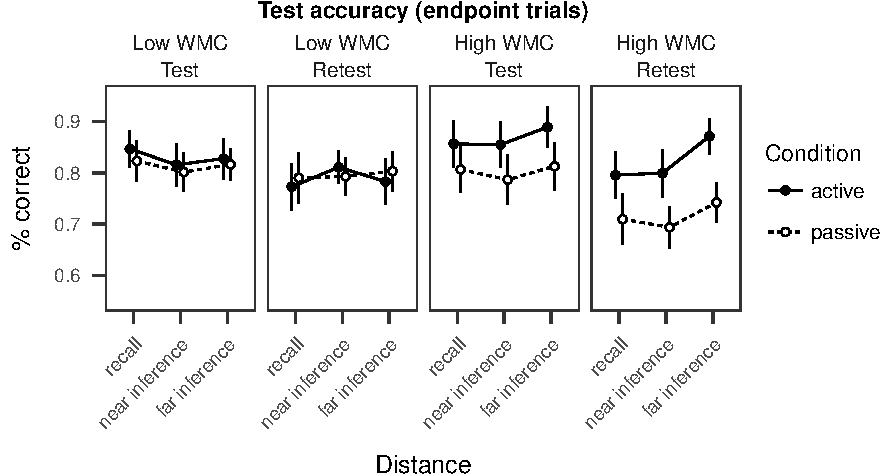
\includegraphics{active_transitive_inference_files/figure-latex/unnamed-chunk-6-1.pdf}
\caption{\label{fig:unnamed-chunk-6}Test accuracy on endpoint trials as a
function of inferential distance and test session, following a median
split on working memory capacity (operation span scores).
\label{fig_acc_endpoint}}
\end{figure}






\end{document}
